\documentclass[a4paper,11pt]{article}
\usepackage[utf8]{inputenc}
\usepackage{lastpage}
\usepackage{fancyhdr}
\usepackage[english]{babel}
\usepackage[a4paper,margin=1in]{geometry}
\usepackage{multirow}
\usepackage[table,xcdraw]{xcolor}
\usepackage{array}
\usepackage{graphicx}
\usepackage{caption}
\usepackage{ctable}
\usepackage{listings}
\usepackage[T1]{fontenc}
\usepackage{bigfoot} % to allow verbatim in footnote
\usepackage[numbered,framed]{matlab-prettifier}
\usepackage{amsmath}

\newcolumntype{L}[1]{>{\raggedright\let\newline\\\arraybackslash\hspace{0pt}}m{#1}}
\newcolumntype{C}[1]{>{\centering\let\newline\\\arraybackslash\hspace{0pt}}m{#1}}
\newcolumntype{R}[1]{>{\raggedleft\let\newline\\\arraybackslash\hspace{0pt}}m{#1}}

\newcommand\tab[1][4mm]{\hspace*{#1}}


%-------------------------------------------------------------------------------
% HEADER & FOOTER
%-------------------------------------------------------------------------------

\pagestyle{fancy}
\fancyhf{}
\setlength\headheight{15pt}
\fancyhead[L]{ Imaging Lab 4 }
\fancyhead[R]{Student ID: 100633486}
\fancyfoot[R]{Page \thepage\ of \pageref{LastPage}}


%-------------------------------------------------------------------------------
% TITLE PAGE
%-------------------------------------------------------------------------------

\begin{document}

\title{
	\Huge \textbf {Nonlinear Filters}
    \\ [0.2cm]
	\LARGE Imaging Lab 4 - May, 2017
    \\ [0.5cm]
    \hrule
}

\date{}

\author{
		\Large Kamyar Nazeri \\
		\large Student ID: 100633486 }

\maketitle
\newpage

\section*{1. Salt \& Pepper Noise, Mean and Median Filters}
To load an image, add 5\% \emph{Salt \& Pepper} noise and apply \emph{Mean} and \emph{Media} filters, we have created a Matlab function (\emph{Process.m}) which takes the ideal image, resizes it to the specified value, adds noise, filters and computes statistics. \\
\emph{Figure 1} shows the \emph{Slat \& Pepper} noise on an image and Mean/Median filters applied on the noisy image:

\begin{figure}[!htb]
  \centering
  
\includegraphics[width=16cm, height=4.8cm]{1.png}
  \caption{\small Salt \& Pepper noise, the mean filtered image and the median filtered image}
\end{figure}

\section*{2. Mean and Median filters: different image sizes}
We use Matlab's \emph{imresize} command to create 4 versions of the original noise-free image with the following sizes: \\
\begin{center}\Large
\textbf{500x500 \tab 1000x1000 \tab 2000x2000 \tab 4000x4000}
\end{center}
 \\The following table shows the runtime of each filter and RMSE/SNR for each filtered image:

\begin{table}[!htb]
\begin{center}
\setlength\extrarowheight{6pt}
\begin{tabular}{|C{2cm}|C{2.4cm}|C{1.5cm}|C{1.5cm}|C{2.4cm}|C{1.5cm}|C{1.5cm}|}
\cline{2-7}
\multicolumn{1}{c|}{\multirow{2}{*}{}}
        & \multicolumn{3}{c}{\textbf{Mean Filter}} & \multicolumn{3}{|c|}{\textbf{Median Filter}} \\ \cline{2-7}
\multicolumn{1}{r|}{}
        & \textbf{Runtime(s)} & \textbf{RMSE} & \textbf{SNR} & \textbf{Runtime(s)} & \textbf{RMSE} & \textbf{SNR} \\ \hline
500x500 & 0.003286 & 0.0371 & 46.9587 & 0.005668 & 0.0272 & 53.1623 \\ \hline
2000x2000 & 0.010378 & 0.0115 & 56.6133 & 0.014682 & 0.0062 & 68.8205 \\ \hline
2000x2000 & 0.053689 & 0.0038 & 64.6637 & 0.059251 & 0.0011 & 88.7440 \\ \hline
4000x4000 & 0.190688 & 0.0017 & 67.229 & 0.210134 & 0.0002 & 107.6343 \\ \hline
\end{tabular}
\caption{Mean/Median filters statistics on different image sizes}
\end{center}
\end{table}

 \\The following shows the Matlab functions to calculate SNR, RSME and a function (Process) to resize an image to the specified value, add noise, filter and compute statistics:

\newpage

\begin{lstlisting}[caption={Matlab SNR Function},captionpos=b,style=Matlab-editor]
function snr = SNR(denoised, ideal)
    % Calculates Signal-to-Noise ratio.
    % Input: Filtered image (denoised). Ideal image (ideal)
    % Output: Scalar snr specifying the SNR of a filter
    snr = 20*log(norm(double(ideal), 'fro')/(norm(double(ideal) - double(denoised), 'fro')));
end
\end{lstlisting}

\begin{lstlisting}[caption={Matlab RMSE Function},captionpos=b,style=Matlab-editor]
function rmse = RMSE(denoised, ideal)
    % Calculates RMS error.
    % Input: Filtered image (denoised). Ideal image (ideal)
    % Output: Scalar rmse specifying the RMSE of a filter
    [m,n] = size(ideal);
    rmse = 1/(m*n)*norm( double(denoised)-double(ideal),'fro');
end
\end{lstlisting}

\begin{lstlisting}[caption={Matlab function to resize an image to the specified value, add noise, filter and compute statistics},captionpos=b,style=Matlab-editor]
function [noisy, mean, mean_rmse, mean_snr, median, median_rmse, median_snr] = Process(img, size)
    % Calculates Lab4 statistics.
    % Input: Image (img). Size of the image (size)

    resized = imresize(img, size);
    median = resized;
    noisy = imnoise (resized, 'salt & pepper', 0.05);
    w = fspecial('average', [5,5]);

    display(['Calculating mean filter ', num2str(size(1))]);
    tic; mean = imfilter(noisy, w, 'replicate'); toc

    display(['Calculating median filter ', num2str(size(1))]);
    tic;
    for i=1:3
        median(:,:,i) = medfilt2(noisy(:,:,i), [5,5]);
    end;
    toc

    resized_gs = rgb2gray(resized);
    mean_gs = rgb2gray(mean);
    median_gs = rgb2gray(median);

    mean_rmse = RMSE(mean_gs, resized_gs);
    mean_snr = SNR(mean_gs, resized_gs);

    median_rmse = RMSE(median_gs, resized_gs);
    median_snr = SNR(median_gs, resized_gs);
end
\end{lstlisting}

\newpage
\section*{Runtime vs. Image Size Visualization}
\emph{Figure 2} shows the runtime vs. the image size plot for mean and median filters:

\begin{figure}[!htb]
  \centering
  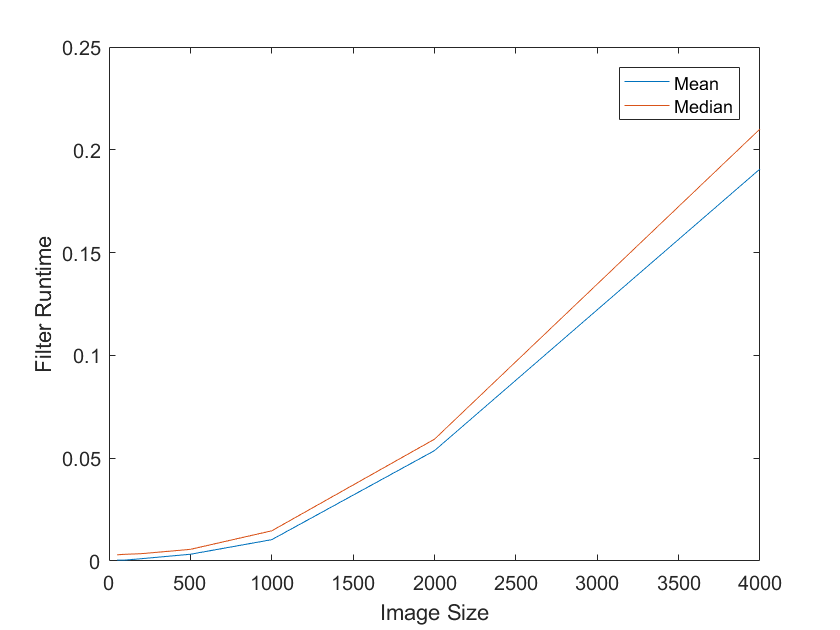
\includegraphics[width=16cm, height=12cm]{2.png}
  \caption{\small Runtime vs. the image size for mean and median filters}
\end{figure}

\section*{Conclusions}
\begin{itemize}
    \item The median filter does a better job on removing salt \& pepper noise as one can visually compare images with mean and median filters in the \emph{figure 1}.
    \item The SNR results in the \emph{Table 1} corroborates previous arguments, note that Signal-Noise-Ratio for Median filter is much higher compared with the results of the Mean filter.
    \item The RMSE error value is decreased with the increase in the size of the image; this is mainly because we applied only 5\% noise on all the sample images, and 5\% noise in smaller images means more noise on the image hence larger error value.
    \item As one can see in \emph{figure 2}, the \emph{Median} filter is generally slower than the \emph{Mean} filter, and the difference in run-time becomes larger with larger image sizes.
\end{itemize}

\end{document}
